% !TEX root = ../../homo_alg.tex

\newpage
\section{Spectral Sequences}
\subsection{Introduction}

Spectral sequences were developed by Leray for use in Algebraic Topology. During World War II, he was imprisoned by the Nazis. Not wanting them to know he was an applied mathematician, he stated he was a pure mathematician who worked in Algebraic Topology. During this time in the war, he developed spectral sequences. These were also independently developed by Lyndon in group cohomology. In 1945, Kozul made the procedure algebraic while in 1952 Massey created exact couples. 

We want to understand the homology of complexes: $H_n(\tot(C_{\cdot \cdot}))$. An example of this would be the calculation of Tor from homologies of individual columns/rows and the maps between them. More generally, $H_n(\dt{C})$, calculating the homology of a complex from parts (meaning subcomplexes and quotients) of it via factors in a filtration of $\dt{C}$ and maps between them. Spectral sequences provide an efficient machinery (more like bookkeeping) to paste these pieces together. 

For some motivation, take a double complex with two columns. 
\begin{figure}[h] 
   \centering
   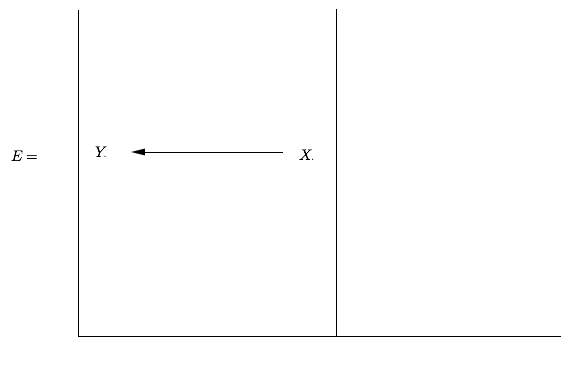
\includegraphics[width=4in]{images/ex1.png} 
\end{figure}

Then $\tot(E)$ is the mapping cone $C(f)$. From the short exact sequence
\[
0 \ma{} Y \ma{} C(f) \ma{} X[-1] \ma{} 0
\]
we get a long exact sequence 
\[
\cdots \ma{} H_{n+1}(X[-1]) \ma{\delta_{n-1}} H_n(Y) \ma{\beta} H_n(C(f)) \ma{\alpha} H_n(X[-1]) \ma{\delta_n} \ma{} \cdots
\]
where $\delta_{n+1}=H_n(f)$, $\delta_n=H_{n-1}(f)$, $H_n(X)=H_{n+1}(X[-1])$, $H_n(C(f))=H_n(\tot(E))$, and $H_{n-1}(X)=H_n(X[-1])$. So we get an exact sequence
\[
0 \ma{} \coker(H_n(f)) \ma{} H_n(\tot(E)) \ma{\alpha} \ker \delta \ma{} 0
\]
where $\ker \delta=\ker(H_{n-1}(f))=\im \text{ previous map}$ and $\coker H_n(Y)/\ker \beta=H_n(V)/\im H_n(f)$. That is, we get a filtration 
\[
H_n(\tot(E)) \supseteq \coker(H_n(f)) \supseteq 0
\]
where factoring yields $\ker(H_{n-1}(f))\cong H_n(\tot(E))/\coker(H_n(f))$ and $\coker(H_n(f)) \cong \coker(H_n(f))/0$. Notice the similarity between this and composition series. Another way to track the same data is to let $E_0=E$, called the $E^0$ or initial page, be given as above. In each position, take homology along the vertical direction to get the $E^1$ page
\[
\begin{tikzcd}
\phantom{x} & \vdots \arrow{d} & \vdots \arrow{d} & \\
0 & H_2(Y) \arrow{l} \arrow{d} & H_2(X) \arrow{l} \arrow{d} & 0 \arrow{l} \\
0 & H_1(Y) \arrow{l} \arrow{d} & H_1(X) \arrow{l} \arrow{d} & 0 \arrow{l} \\
0 & H_0(Y) \arrow{l} \arrow{d} & H_0(X) \arrow{l} \arrow{d} & 0 \arrow{l} \\
 & 0 & 0 & \\
\end{tikzcd}
\]
where the vertical maps are now 0, so they are no longer useful. However, the horizontal maps still carry useful information. So we take horizontal homology to get the $E^2$ page
\[
\begin{tikzcd}
\phantom{x} & \vdots \arrow{d} & \vdots \arrow{d} & \\
0 & \coker(H_2(f)) \arrow{l} \arrow{d} & \ker(H_2(f)) \arrow{l} \arrow{d} & 0 \arrow{l} \\
0 & \coker(H_1(f)) \arrow{l} \arrow{d} & \ker(H_1(f)) \arrow{l} \arrow{d} & 0 \arrow{l} \\
0 & \coker(H_0(f)) \arrow{l} \arrow{d} & \ker(H_0(f)) \arrow{l} \arrow{d} & 0 \arrow{l} \\
 & 0 & 0 & \\
\end{tikzcd}
\]
where now the horizontal maps are useful. However, we have maps along the diagonal (that is, along the lines $y= n-x$ for $n \in \Z \cup \{0\}$. But these turn out to be not useful. Taking homology along these diagonal lines changes nothing so we have
\[
E^2=E^3=E^4=\cdots=E^\infty
\]
Notice how we took the various maps
\begin{figure}[h] 
   \centering
   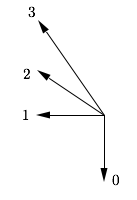
\includegraphics[width=1in]{images/maps.png} 
\end{figure}
Recall $H_n(\tot(E))$ has filtration with factors $\coker(H_n(f)), \ker H_{n-1}(f))$ which are in $E_2$ above (if we took $\tot$ with $p+q=n$, considering $(p,q)=(x,y)$). This is an interesting connection. 

As another example, take $E=E^0$ the bicomplex with differentials $d^V$ the vertical maps and $d^H$ the horizontal maps. To find $H_n(\tot(E))=Z_n/B_n$, we need to find the cycles. 
\begin{figure}[h] 
   \centering
   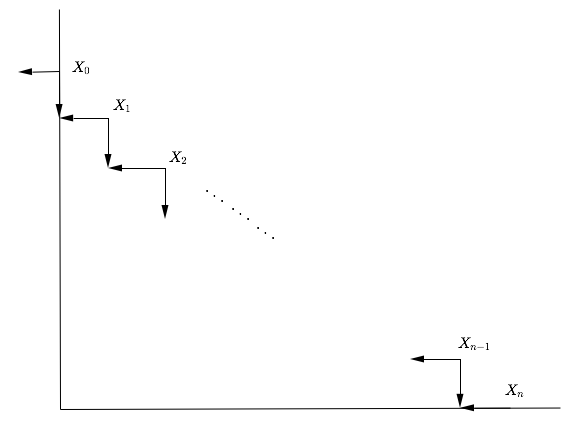
\includegraphics[width=3in]{images/diagonal.png} 
\end{figure}
That is, we want to find ordered tuples $x+y=n, i+j=n, p+q=n$, $\oplus_{p+q=n} E_{p,q}$ with $d^V(X_p)=d^H(X_{p+1})$ (so that they cancel out) and $d^H(X_0)=0$ and $d^V(X_n)=0$. But how do we do this? We start with $x_n \in \ker d^V$ so that $\overline{x_n} \in H_0(\text{column})$. Let $z_n=d^H(x_n)$. Now we have $Z_n=d^V(\text{some }x_{n-1})$ if and only if $z_n \in \im d^V$ if and only if $\overline{z}_n=0$ in $H_0(\text{column }n-1)$ if and only if $\overline{x}_n \in \ker(H_0(\text{column }n) \to H_0(\text{column }n-1)$. If so, we can assign to the $x_n$ the element $x_{n-1}$ and look at the $Z_{n-1}=d^H(X_{n-1})$, where the maps go between the $X_n$ two left and one up. Note throughout we have dropped $\pm$ on elements to make things work for simplification. That is, we take ``$\overline{x}_n \in H^H(H^V(\text{column}))$". So $E^1$ is the bicomplex with vertical homologies in $E^0$ and $E^2$ is the bicomplex with the horizontal homology of $E^1$. Continuing this process, one can see any element $\overline{x}_n$ surviving in spot $(p,q)=(n,0)$ on page $E^n$ can be represented by an $x_n$ that can be extended to give a cycle $(x_0,\cdots,x_n)$ in the original $H_n(\tot(E))$ with arrows $(r,0) \mapsto (r,r-1)$.

\subsection{Homology Spectral Sequence}

\begin{dfn}[(Homology) Spectral Sequence]
A (homology, so the arrows go down and left, that is not a cochain complex) spectral sequence in an abelian category $A$ is 
\begin{enumerate}[(i)]
\item a family of pages: $E^r=\{E_{p,q}^r\}$ of objects for all $p,q \in \Z$, $r \geq r_0$, i.e. the start page.
\item in each page, $E^r$ has maps $d^r: E_{p,q}^r \to E_{p-r,q+(r-1)}^r$ with $(d^r)^2=0$.
\item the objects in page $E^{r+1}$ satisfy $E^{r+1}_{p,q} \cong H_{p,q}(E^r,dr)$. That is, the homology of the previous page in each spot. 
\end{enumerate}
\end{dfn}

It is important to note that though we can draw $E^0$ in a grid with $d^0$, this does not have to be a bicomplex. Furthermore, note that $E^{r+1}_{p,q}$ is a sub quotient, i.e. a quotient of a submodule of $E^r_{p,q}$. So one might ask if the $E^{r+1}$ page inherits any properties from the $E^r$ page. This also shows that the $E$'s are only getting ``smaller". In fact, at any spot $(p,q)$ we have (via the Correspondence Theorem)
\[
0=B^{r_0}_{p,q} \subseteq \cdots \subseteq B^r_{p,q} \subseteq B^{r+1}_{p,q} \subseteq \cdots \subseteq Z_{p,q}^{r+1} \subseteq Z^r_{p,q} \subseteq \cdots \subseteq Z_{p,q}^{r_0} = E_{p,q}^r
\]
where the sequence of $B$'s are images of arrows lifted to $E_{p,q}^0$ with $B^r_{p,q}/Z_{p,q}^r \cong E_{p,q}^r$ in $E_0$.

\begin{dfn}
A spectral sequence is bounded if for each $n$, the ``$p+q=n$" diagonal has finitely many nonzero entries. 
\end{dfn}

Note that if a spectral sequence is bounded, the differentials $d^r$ coming in and out of each spot will eventually be zero maps. Why?
\[
E_{p+r,q-(r-1)}^r \ma{} E_{p,q}^r \ma{} E_{p-r,q+(r-1)}
\]
with sums $n+1,n,$ and $n-1$ respectively, will be 0 for large $n$. So $E^r_{p,q}=E_{p,q}^{r+1}=E_{p,q}^{r+2}=\cdots$. We call this minimal $r$ such that this occurs the stable value $E^\infty_{p,q}$. If the spectral sequence is not bounded, we have to do other things:
\[
E^\infty_{p,q} = \frac{\bigcap_r Z^r_{p,q}}{\bigcup_r B^r_{p,q}}
\]

\begin{dfn}
We say a spectral sequences converges to objects $\{H_n\}$ if for each $n$, the objects $\{E^\infty_{p,q} \;|\; p+q=n\}$ give factors in some filtration of $H_n$, written $E^{r_0}_{p,q} \to H_{p+q}$ or $E^{r_0}_{p,q} \to H_n$.
\end{dfn}

But this is useless unless $\{H_n\}$ is relevant to something about the original set-up used to make the spectral sequence, e.g. $E^0$ or something about the $E^0$ page. 

\subsection{Cohomology Spectral Sequence}

Now we define the dual version:

\begin{dfn}[(Cohomology) Spectral Sequence]
A (cohomology) spectral sequence is
\begin{enumerate}[(i)]
\item family of pages $E_r=\{E_r^{p,q}\}$ for all $p,q \in \Z$ and $r \geq r_0$
\item on each page, maps $d_r: E_r^{p,q} \to E_r^{p+q,q-(r-1)}$ with $(d_r)^2=0$.
\item $E_{r+1}^{p,q}=H_{p+q}(E_r^{p,q},d_r)$ (that is the homology of the previous page at the spot $p,q$).
\end{enumerate}
\end{dfn}

Note that if you reindex $E^{p,q}$ as $E_{p,-q}$ then this is the old definition of a homology spectral sequence. This shows that proving theorems for the homology spectral sequences shows them by a dual argument for the cohomology spectral sequence. 

\begin{dfn}
We say that $\{E_r^{p,q}\}$ is bounded if in each diagonal $p+q=n$, there are finitely many nonzero objects. If so, then eventually $E_r^{p,q}=E_{r+1}^{p,q}=\cdots$. We call this the stable value $E_\infty^{p,q}$. The spectral sequence converges to $\{H^n\}$ if for each $n$, objects in the diagonal $p+q=n$ are the factors in some filtration of $H^n$. We write $E_r^{p,q} \to H^{p+q}$ or $H^n$.
\end{dfn}

\begin{ex}
Any $\{E^{p,q}\}$ spectral sequence converges to $E^{p,q}_r \to \oplus_{p+q=n} E^\infty_{p,q} \defeq H_n$. That is,
\[
H^n \supseteq * \supseteq * \supseteq \cdots \supseteq 
\]
with factors $E_\infty^{s,n-s}$, $E_\infty^{p,n-p},\cdots, E^{\text{last}}_\infty$. We have a reversed conclusion for a cohomology spectral sequence. 
\end{ex}

\subsection{Filtrations and Bounded Spectral Sequences}

We have some ``inclusion" of spectral sequences:
\[
\text{General Spectral Sequence} \supseteq \text{Filtration Spectral Sequence} \supseteq \text{Spectral Sequence of a Double Complex}
\]
The Loray-Serre spectral sequence of a fibration is a type of filtration of a spectral sequence: if $F$ is a fiber ($\pi^{-1}(b)$ for some $b \in B$) and $B$ is the base
\[
F \ma{} E \ma{\pi} B
\]
We will see how from a complex $C$ with a filtration by subcomplexes to construct a spectral sequence from the homology of the factors converges to the homology of $C$. 

\begin{dfn}[Filtration]
A filtration of a chain complex $\dt{C}$ is a chain of subcomplexes 
\[
\cdots \subseteq F_{p-1}C \subseteq F_pC \subseteq \cdots \subseteq C
\]
\end{dfn}

We will assume that the filtration is bounded (any position in the complex eventually stabilizes for all $n$, i.e. there are only finitely many $(F_pC)_n \neq 0$) or bounded below or exhaustive:
\[
\bigcup_p F_pC = C
\]
Now we look at the construction of the filtration. 

\begin{figure}[h] 
   \centering
   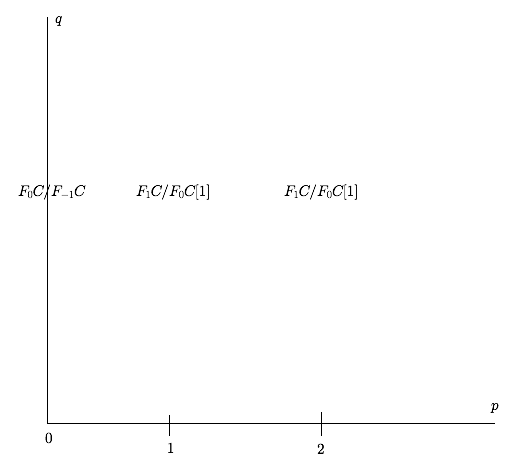
\includegraphics[width=4in]{images/grid.png} 
\end{figure}

Let $E^0_{p,q}=(F_pC/F_{p-1}C)_{p+q}=F_pC_{p+q}/F_{p+1}C_{p+q}$. That is, the $p$th column is the $p$th factor shifted down by $p$-steps. The differential $d$ on $C$ induces vertical maps (differential of factor complex $d^0: E^0_{p+q} \to E^0_{p,q-1}$). We know that $E^1_{p,q}=H_{p+q}(F_pC/F_{p-1}C)$. For the page $r$ (dropping the $p+q$ subscripts), let $\pi_p: F_pC \to F_pC/F_{p-1}C=E_p^0$ and $A^r_p=\{x \in F_pC \;|\; d(x) \in F_{p-r}C \}$, which are the ``cycles modulo $F_{p-r}C$". Then $Z_p^r=\pi(A_p^r) \supseteq B_p^r=\pi(d(A^{r-1}_{p+r-1}))$. We have $Z_p^r,B_p^r \subseteq F_pC/F_{p+1}C$. Note that we have
\[
0=B^0_p \subseteq B_p^1 \subseteq \cdots \subseteq B_p^r \subseteq \cdots \subseteq Z_p^r \subseteq \cdots \subseteq Z_p^1 \subseteq Z_p^0=E_p^0
\]
and let $E^r_p=Z^r/B_p^r \cong A^r_p/\left(d(A^{r-1}_{p+r-1})+A^{r-1}_{p-1}\right)$ (the congruence follows from the Second Isomorphism Theorem). Define $d^r$ to be the map induced by the original differential of $C$. One need check $(d^r)^2=0$ and $E^{r+1} \cong H(E^r,d^r)$. We have the following difficult (though not deep) Theorem:

\begin{thm}[Convergence Theorem]
If the filtration on $C$ is bounded or bounded below and exhaustive then the spectral sequence constructed above converges (this is trivial as it is bounded) to the homology of $C$: $E_{p,q}^1=H_{p+q}(F_p/F_{-1}) \to H_{p+q}(C)$. 
\end{thm}

We have the special case of the spectral sequence of a double complex. Then $\tot(C_{\cdot \cdot})$ has (at least) two canonical filtrations. The first is
\begin{figure}[h] 
   \centering
   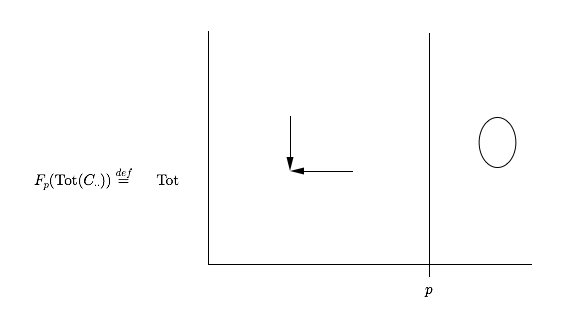
\includegraphics[width=4in]{images/almostfinal.png} 
\end{figure}
Note $E^0_{p,q} \defeq F_p/F_{p-1}= \text{column }p \text{ of } C_{\cdot \cdot}$ with $d^0$ the vertical differential $d^V$. We have $E^1_{p,q}=H^V_q(C_{p,*})$ and $d^1$ the differential induced by the original horizontal differential $d$ of $\tot(C_{\cdot \cdot})$ which is the horizontal differential induced by $d^H$ of $C_{\cdot \cdot}$ on the sub quotients (since $d^V(x)=0$ for all $\overline{x} \in H^V(C_{\cdot \cdot})$. So $E^2_{p,q}=H^H_pH^V_q(C)$. By the Convergence Theorem, we have $E^2_{p,q}=H^H H^V_q(C) \to H_{n=p+q}(\tot(C_{\cdot \cdot})$. The canonical construction follows similarly by exchanging the roles of $p,q$. 

\begin{figure}[h] 
   \centering
   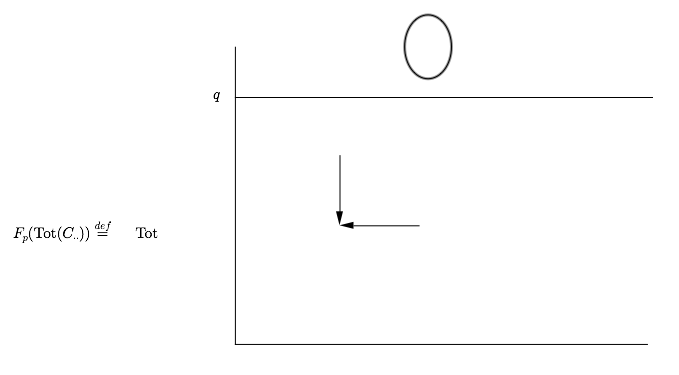
\includegraphics[width=4in]{images/final.png} 
\end{figure}













